\documentclass[11pt]{report}
\usepackage{fullpage}
\usepackage{graphics}
\usepackage{tabularx}

\usepackage{times}
\usepackage{listings}
\lstset{language=C,basicstyle=\footnotesize,frame=tb}

\def\VERSION {1.5}
\def\DEFAULTPORT {6665}
\def\HOMEPAGE {{\tt http://playerstage.sourceforge.net}}
\def\libplayerc {{\tt libplayerc} }

\begin{document}
\setcounter{page}{0}
\pagenumbering{roman}

\titlepage

\begin{tabular}{lcr}
  \begin{tabular}{c}
	Player/Stage project\\
        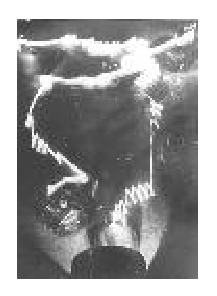
\includegraphics{notext_ps_logo}
   \end{tabular}
  &
  \hspace{5cm}
  &
  \begin{tabular}{r}
    {\bf USC Robotics Laboratory}\\
    University of Southern California\\
    Los Angeles, California, USA\\
  \end{tabular}
\end{tabular}

\vspace{5cm}
\centerline{\huge{libplayerc}}
\vspace{0.5cm}
\centerline{\large{Version \VERSION\ Reference Manual}}
\vspace{2cm}

\centerline{\large Andrew Howard}
\centerline{\sl ahoward@usc.edu}
\vspace{5cm}
\centerline{\today}

\newpage
\tableofcontents

\newpage
\setcounter{page}{0}
\pagenumbering{arabic}

\chapter{Introduction}

\libplayerc is a client library for the Player robot device server.
It is written in C to maximize portability, and in the expectation
that users will write bindings for other languages (such as Java)
against this library; Python bindings for \libplayerc are already
available.

Users reading this manual this manual should also read the {\em Player
User Manual} included in the standard Player distribution.


\section{Getting \libplayerc}

\libplayerc is included with the standard Player distribution, starting with
version 1.2.  The Player homepage is:
\begin{quote}
\HOMEPAGE
\end{quote}
Check there for the latest versions of the Player distributon and this
document.  The default Player installation will build and install the
following files:
\begin{quote}
\begin{verbatim}
$(HOME)/player-1.3/include/playerc/playerc.h
$(HOME)/player-1.3/lib/playerc/libplayerc.a
\end{verbatim}
\end{quote}
Make sure these directories are in your include and library paths,
respectively.


\section{Differences between versions 1.2 and 1.3}

(Users who are familiar with version 1.2 of \libplayerc should read
this section; new users may safely ignore it).

The Player server has been substantially re-written to support a more
general interface/driver model for devices.  A device {\em interface}
describes the kinds of interactions a device allows, while a device
{\em driver} handles the low-level hardware interaction.  Thus one may
use the same interface to control many different pieces of hardware,
each of which has a specific driver.

This change has two important consequences for the \libplayerc client
library:
\begin{itemize}
\item Client-side {\em proxies} now correspond to server-side {\em
interfaces}.  Thus, for example, a {\tt position} proxy on the client
connects to a {\tt position} interface on the server.
\item Some proxy names have changed to bring them into line with the
new server naming conventions.
\end{itemize}
See the {\em Player User Manual} for more details on the new
interface/driver model.


\section{Bugs}

This software is provided WITHOUT WARRANTY.  Nevertheless, if you find
something that doesn't work, or there is some feature you would like
to see, you can submit a bug report/feature request through the
Player/Stage homepage:
\begin{quote} 
\HOMEPAGE
\end{quote}
Include a detailed description of you problem and/or feature request,
and information such as the Player version and operating system.  Make
sure you also select the ``\libplayerc'' category when reporting bugs.


\section{Licence}

This program is free software; you can redistribute it and/or modify
it under the terms of the GNU General Public License as published by
the Free Software Foundation; either version 2 of the License, or (at
your option) any later version.  This program is distributed in the
hope that it will be useful, but WITHOUT ANY WARRANTY; without even
the implied warranty of MERCHANTABILITY or FITNESS FOR A PARTICULAR
PURPOSE.  See the GNU General Public License for more details.  You
should have received a copy of the GNU General Public License along
with this program; if not, write to the Free Software Foundation,
Inc., 59 Temple Place - Suite 330, Boston, MA 02111-1307, USA.

\section{Acknowledgements}

This work is supported by DARPA grant DABT63-99-1-0015 (MARS) and NSF
grant ANI-9979457 (SCOWR), and possibly others.


\chapter{General Usage}

\libplayerc is based on a device ``proxy'' model, in which the client
maintains a local proxy for each of the devices on the remote server.
Thus, for example, one can create local proxies for the {\tt position}
and {\tt laser} devices.  There is also a special {\tt client} proxy,
used to control the Player server itself.  

Programs using \libplayerc will generally the following structure:
\begin{quote}
\begin{lstlisting}[frame=tb]{}
#include <stdio.h>
#include "playerc.h"

int main(int argc, const char **argv)
{
  int i;
  playerc_client_t *client;
  playerc_position_t *position;

  client = playerc_client_create(NULL, "localhost", 6665);
  playerc_client_connect(client);

  position = playerc_position_create(client, 0);
  playerc_position_subscribe(position, PLAYER_ALL_MODE);

  playerc_position_enable(position, 1);
  playerc_position_set_speed(position, 0, 0, 0.1);
  
  for (i = 0; i < 200; i++)
  {
    playerc_client_read(client);
    printf("position : %f %f %f\n",
           position->px, position->py, position->pa);
  } 

  playerc_position_unsubscribe(position);
  playerc_position_destroy(position);
  playerc_client_disconnect(client);
  playerc_client_destroy(client);

  return 0;
}
\end{lstlisting}
\end{quote}
Note that error checking has been omitted from this example for the
sake of clarity (for an example with full error checking, see {\tt
simple.c} in the {\tt examples/libplayerc} directory).  This example
can be built using the commands:
\begin{quote}
\begin{verbatim}
$ gcc -c simple.c -o simple.o
$ gcc -lm -lplayerc simple.o -o simple
\end{verbatim}
\end{quote}
Make sure that {\tt playerc.h} is in you include path, and that {\tt
libplayerc.a} is in your library path.

The above program can be broken into six steps, as follows.

\subsection*{Create and connect a client proxy.}

\begin{quote}\begin{verbatim}
client = playerc_client_create(NULL, "localhost", 6665);
playerc_client_connect(client);
\end{verbatim}\end{quote}
The {\tt create} function creates a new client proxy and returns a
pointer to be used in future function calls ({\tt localhost} should be
replaced with the network host name of the robot).  The {\tt connect}
function notifies the Player server that a new client wishes to
recieve data.

\subsection*{Create and subscribe a device proxy.}

\begin{quote}\begin{verbatim}
position = playerc_position_create(client, 0);
playerc_position_subscribe(position, PLAYER_ALL_MODE);
\end{verbatim}\end{quote}
The {\tt create} function creates a new position device proxy and
returns a pointer to be used in future function calls.  The {\tt
subscribe} function notifies the Player server that the client is
using the position device, and that the client expects to both send
commands and recieve data ({\tt PLAYER\_MODE\_ALL}).

\subsection*{Configure the device, send commands.}

\begin{quote}\begin{verbatim}
playerc_position_enable(position, 1);
playerc_position_set_speed(position, 0, 0, 0.1);
\end{verbatim}\end{quote}
The {\tt enable} function sends a configuration request to the server,
changing the robot's motor state from {\tt off} to {\tt on}, thereby
allowing the robot to move.  The {\tt setspeed} function sends a new
motor speed, in this case commanding the robot to turn on the spot.

Note that most Player devices will accept both asynchronous {\em
command} and synchronous {\em configuration} requests.  Sending
commands is analogous using the standard Unix {\tt write} device
interface, while sending configuration requests is analogous to using
the {\tt ioctl} interface.  For the most part, {\tt libplayerc} hides
the distinction between these two interfaces.  Users should be aware,
however, that while commands are always handled promptly by the
server, configuration requests may take significant time to complete.
If possible, configuration requests should therefore be restricted to
the initialization phase of the program.

\subsection*{Read data from the device.}

\begin{quote}\begin{verbatim}
playerc_client_read(client);
printf("position : %f %f %f\n", position->px, ... );
\end{verbatim}\end{quote}
The {\tt read} function blocks until new data arrives from the Player
server.  This data may be from one of the subscribed devices, or it
may be from the server itself (which sends regular synchronization
messages to all of its clients).  The {\tt read} function inspects the
incoming data and automatically updates the elements in the
appropriate device proxy.  This function also returns a pointer to the
proxy that was updated, so that user programs may, if desired, trigger
appropriate events on the arrival of different kinds of data.

\subsection*{Unsubscribe and destroy the device proxy.}

\begin{quote}\begin{verbatim}
playerc_position_unsubscribe(position);
playerc_position_destroy(position);
\end{verbatim}\end{quote}
The {\tt unsubscribe} function tells the Player server that the client
is no longer using this device.  The {\tt destroy} function then frees
the memory associated with the device proxy; the {\tt device} pointer
is now invalid and should be not be re-used.

\subsection*{Disconnect and destroy the client proxy.}

\begin{quote}\begin{verbatim}
playerc_client_disconnect(client);
playerc_client_destroy(client);
\end{verbatim}\end{quote}
The {\tt disconnect} function tells the server that the client is
shutting down.  The {\tt destroy} function then frees the memory
associated with the client proxy; the {\tt client} pointer is now
invalid and should be not be re-used.



\chapter{Library Reference}

This chapter contains information on the various non-device and
generic proxies offered by \libplayerc; see Chapter \ref{chap.devices}
for information on specific device proxies.

%\section{The {\tt client} proxy}
%
%The client proxy provides an interface to the Player server itself,
%and therefore has somewhat different functionality from the {\em
%device} proxies.  The client proxy supports the following functions:
%\begin{quote}
%\lstinputlisting{client.f.tex}
%\end{quote}
%Note that the {\tt create} function returns a pointer to an {\tt
%playerc\_client\_t} structure to be used in other function calls.
%This structure is opaque and should not be manipulated directly.

%\newpage
\input{proxies/client}

%\section{The {\tt device} proxy}
%
%The {\tt device} proxy provides a `generic' interface to the
%functionality that is shared by all devices (i.e., a base class, in
%OOP parlance).  This proxy can be accessed through the {\tt info}
%element present in each of the device proxies; {\tt info} is of type
%{\tt playerc\_device\_t}, and has the following elements:
%\begin{quote}
%\lstinputlisting{device.t.tex}
%\end{quote}
%The elements that are marked are ``private'' should are reserved for 
%internal use and should not be manipulated directly.

%\newpage
\input{proxies/device}

%\section{Error handling}
%
%Most functions in \libplayerc will return 0 on success and non-zero
%value on error.  A descriptive error message will also be written into
%the error variable:
%\begin{quote}
%\begin{lstlisting}{}
%char *playerc_errorstr;
%\end{lstlisting}
%\end{quote}


%\newpage
\input{proxies/Errors}


\chapter{Device Reference}
\label{chap.devices}

This chapter contains information on the various types of proxies
offered by \libplayerc: each type of proxy corresponds to one of the
{\em interface} types offered by the Player server.  Note that this
section is not intended to provide a complete reference for all of the
devices offered by Player, and should be read in conjunction with the
Player User Manual.


\section{Units}

Unless otherwise specified, proxies use SI units (meters, radians,
seconds) for all measurements.

\section{Device Summary}

\libplayerc has proxies for the following devices:

\noindent
\begin{tabularx}{\columnwidth}{lX}
\hline
{\tt blobfinder} & Color-blob detector: an interface to a color blob detectors such as the
ACTS vision system.\\
{\tt comms} & Broadcast communications device: sends and receives packets between Player
clients via the server.\\
{\tt laser} & Laser device: interface for scanning laser range-finders
such as the SICK LMS200.\\
{\tt localize} & Localization device: returns the global robot pose.\\
{\tt fiducial} & Fiducial detector: detects fiducials (beacons) placed in the
environment.\\
{\tt position} & Position device: for control of a mobile robot platform.\\
{\tt power} & Power device: query batter levels.\\
{\tt ptz} & Pan-tilt-zoom device: an interface to a pan-tilt-zoom camera
head such as the Sony EVID30 \\
{\tt sonar} & Sonar device: an interface to an array of sonar range finders, 
such as those built into a mobile robot base.\\
{\tt truth} & Truth device: allows clients to get and set the pose of
objects in the Stage simulator.  {\bf Simulator only.}\\
{\tt wifi} & WiFi device: queries link status on wireless networks.\\
\hline
\end{tabularx}

\newpage
\input{proxies/blobfinder}

\newpage
\input{proxies/comms}

\newpage
\input{proxies/fiducial}

%\newpage
%\input{proxies/gps}

\newpage
\input{proxies/laser}

\newpage
\input{proxies/localize}

\newpage
\input{proxies/position}

\newpage
\input{proxies/power}

\newpage
\input{proxies/ptz}

\newpage
\input{proxies/sonar}

\newpage
\input{proxies/truth}

\newpage
\input{proxies/wifi}



\appendix

\chapter{Complete Header Listing}

This is a complete listing of {\tt playerc.h}.

\lstinputlisting{../playerc.h}

\end{document}


